\documentclass[article,A4,12pt]{llncs}
\usepackage[T1]{fontenc}
\usepackage{amsmath}
\usepackage{amssymb}
\usepackage{amsfonts}
\usepackage{mathrsfs, bm}

\usepackage{graphicx}
\usepackage{tabularx}
\usepackage{subfig}
\usepackage{epsf,times}
\usepackage{color}
\usepackage{wrapfig}
\usepackage{cases}
\usepackage{multicol}

\usepackage[T1]{fontenc}
%\newcommand{\tmname}[1]{\textsc{#1}}
%\newcommand{\tmop}[1]{\ensuremath{\operatorname{#1}}}
%\newcommand{\tmsamp}[1]{\textsf{#1}}
%\newcommand{\tmtextsc}[1]{{\scshape{#1}}}
%\newcommand{\tmtextsl}[1]{{\slshape{#1}}}
%\newcommand{\tmtexttt}[1]{{\ttfamily{#1}}}

\leftmargin=0.0cm
\oddsidemargin=0.5cm
\evensidemargin=0.5cm
\topmargin=0cm
\textwidth=16.0cm
%\textheight=21.5cm
\textheight=20.0cm
\pagestyle{plain}
\setlength{\columnsep}{20pt}

\def\m{\mathbf{m}}
\def\H{\mathbf{H}}
\def\E{\mathbf{E}}
\newcommand{\vepsi}{{\varepsilon}}
\def\hnorm#1#2{\vert\,#1\,\vert_{#2}}
\newcommand{\R}{{\mathbb R}}
\newcommand{\Sph}{{\mathbb S}}
\def\x{\mathbf{x}}
\def\hvec{\overline{\mathbf{h}}}
\def\evec{\overline{\mathbf{e}}}

\newcommand{ \etal}{\mbox{\emph{et al. }}}

\newcommand\vect[1]{\mbf{#1}}
\newcommand{\mbf}[1]{\mbox{\boldmath$#1$}} 
\newcommand{\RC}[1]{#1 $\times$ #1 $\times$ #1}
\def\um{$\mu$m}
\def\C{$^{\circ}\mathrm{C}$}

\newcommand{\Rmnum}[1]{\expandafter\@slowromancap\romannumeral #1@}

% DEFINITION OF CUSTOM FONT SIZE
\newcommand{\customfontA}{\fontsize{50}{55}\selectfont}
\newcommand{\customfontB}{\fontsize{14.4}{20}\selectfont}
\newcommand{\customfontC}{\fontsize{30}{35}\selectfont}

\DeclareMathAlphabet{\mathpzc}{OT1}{pzc}{m}{it}

\def\clovek#1{\noindent\bgroup\vbox{\noindent#1}\egroup\vskip1em}

% TO INPUT BACKGROUND IMAGE
\usepackage{eso-pic}
\newcommand\BackgroundPic{
\put(0,0){
\parbox[b][\paperheight]{\paperwidth}{
\vfill
\centering
\includegraphics[width=\paperwidth,height=\paperheight]{img/plasm-frontpage.png}
%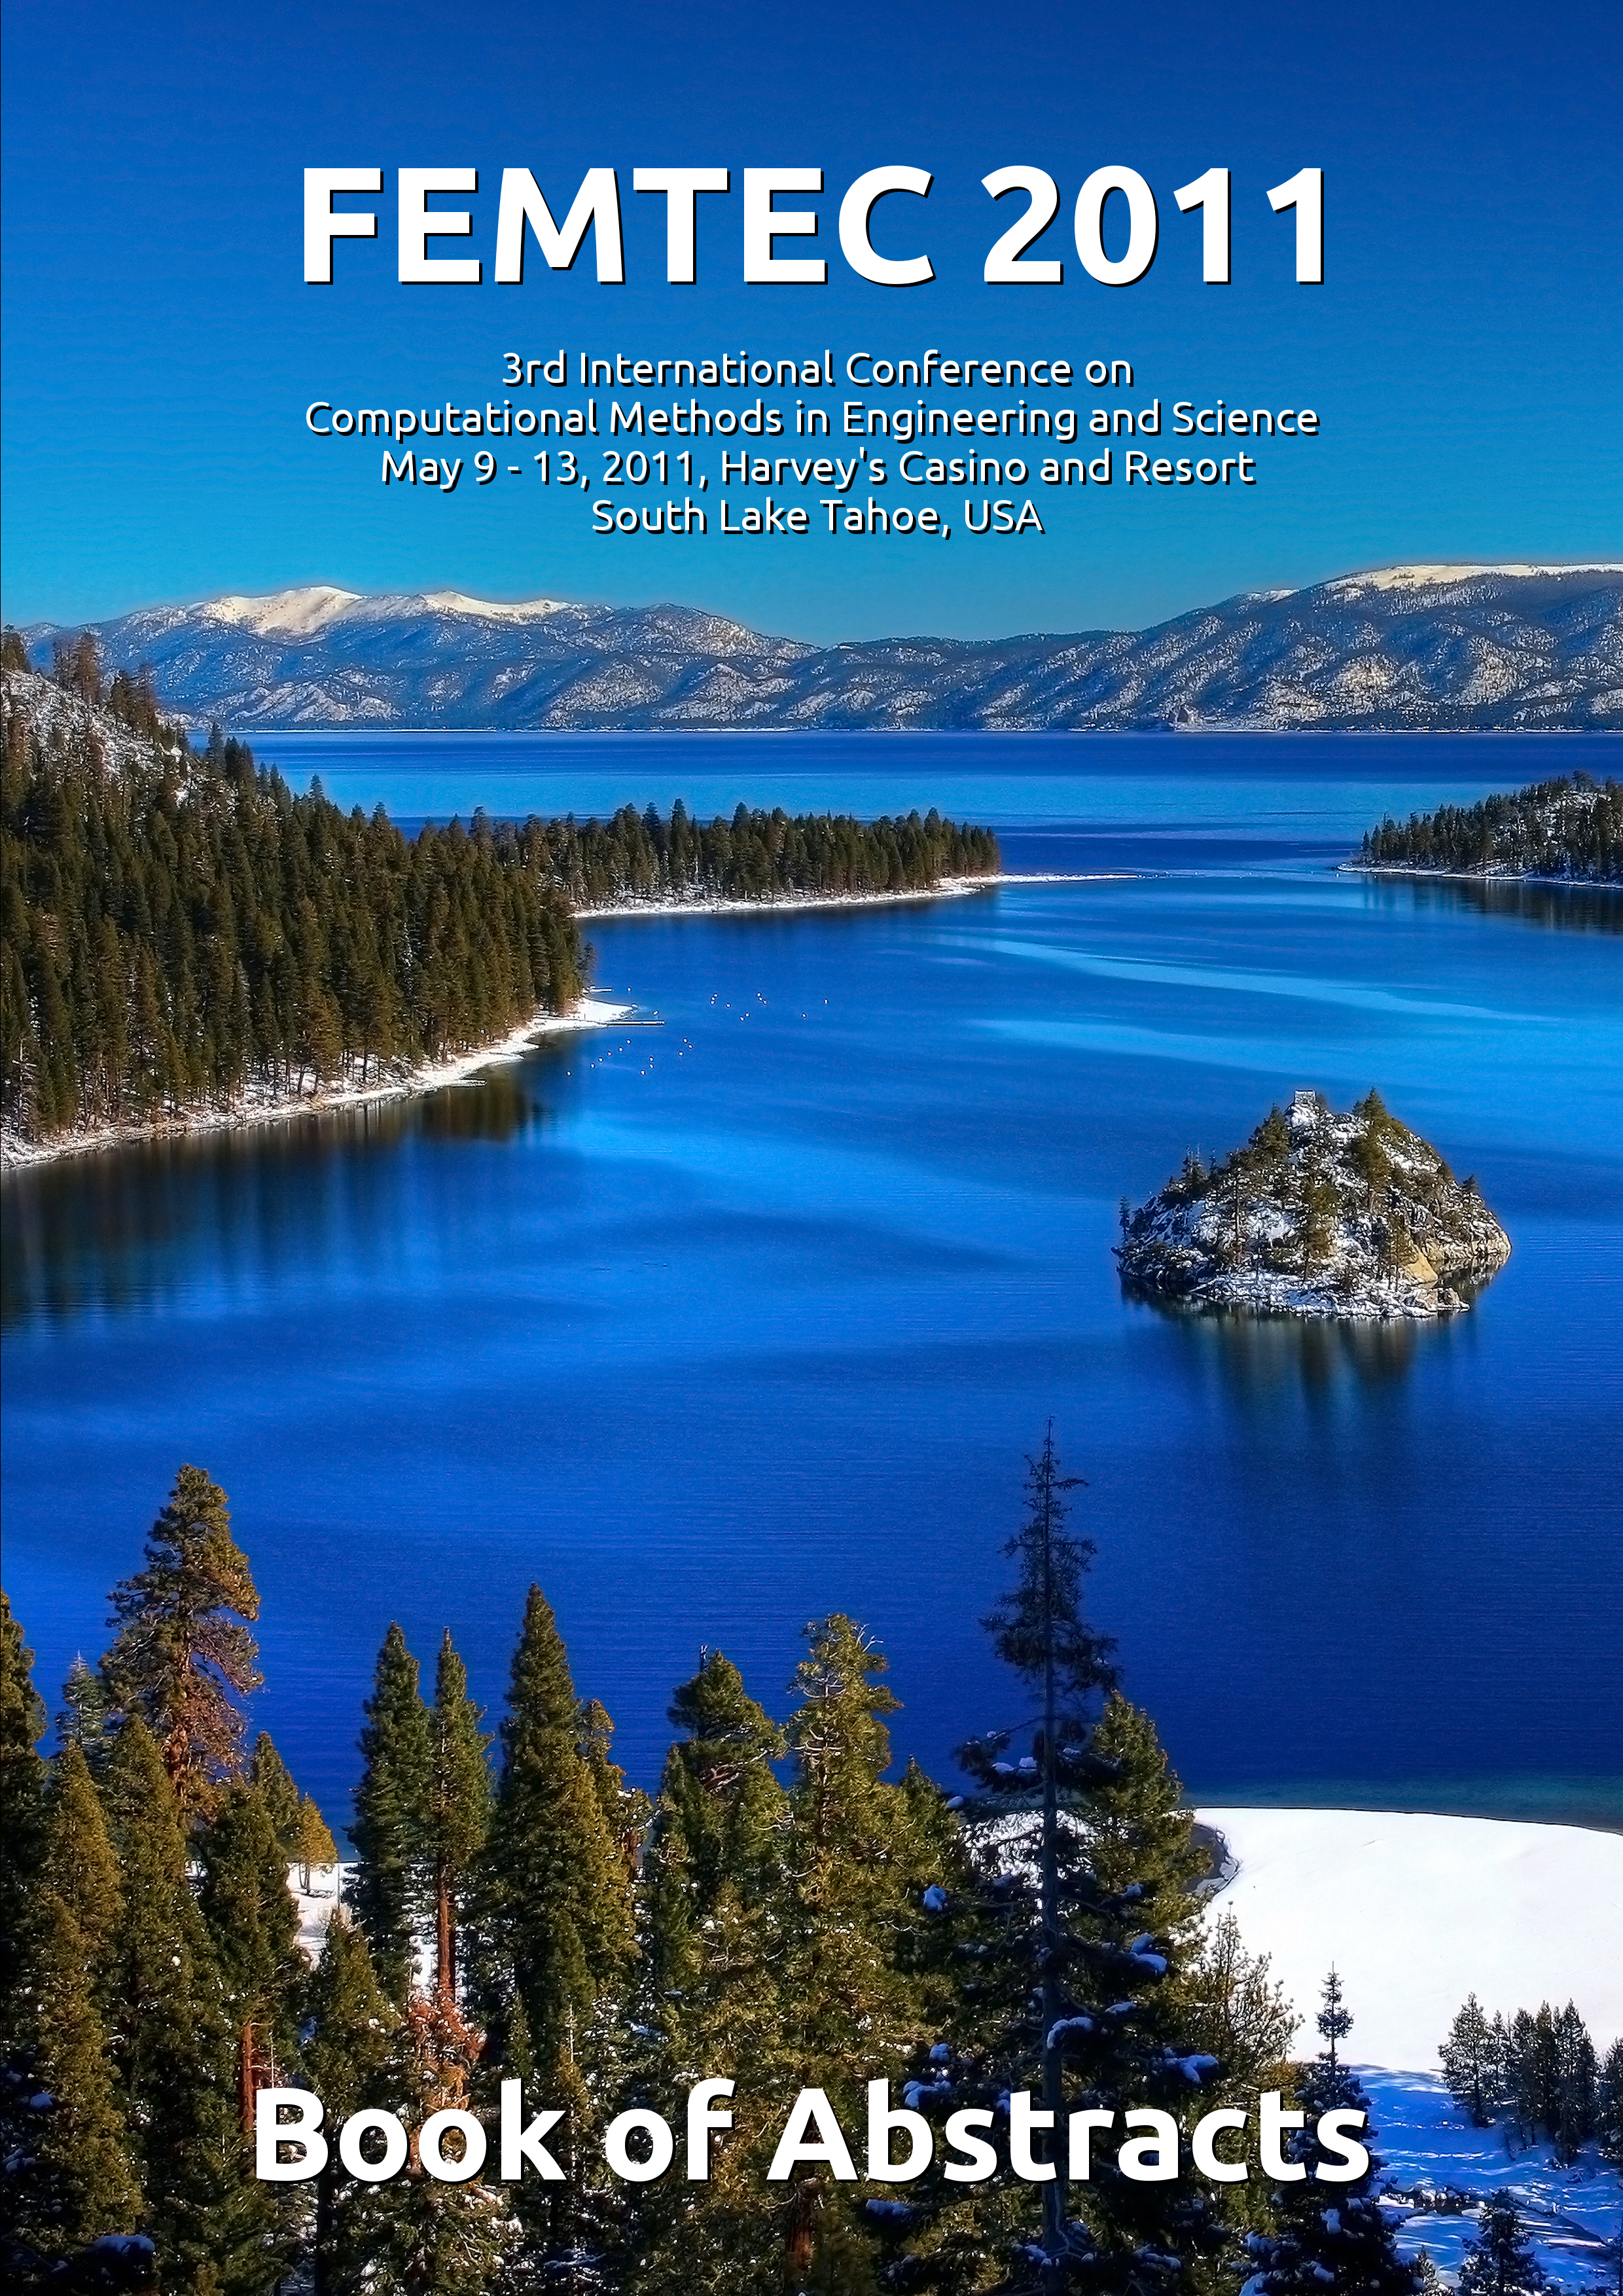
\includegraphics[width=\paperwidth,height=\paperheight]{img/background.jpg}
\vfill
}}}

\begin{document}

% INPUTTING BACKGROUND IMAGE
\AddToShipoutPicture{\BackgroundPic}
\vbox{}
\pagestyle{empty}
\newpage
\textwidth=15.5cm
\ClearShipoutPicture
\newpage

%%%%%%%%%%%%%%%%%%%%%%%%%%%%%%%%%%%%%%%%%%%%%%%%%%%%%%%%%%%%%%%%%%%%%%%%%

\section*{}
\small
\subsection*{About NCLab}
Networked Computing Laboratory (NCLab) is a popular Internet-based framework for 
programming, mathematics, computer modeling, 
and scientific computing. It serves students, instructors, researchers, and the general 
public. NCLab can be used free of charge for personal non-commercial purposes such as 
private hobby or self-education, as well as for individual non-funded academic research.
All other use is subject to {\bf purchasing a license} for a symbolic fee. The fees are as low as 
\$1 per user per month for educational use, and they are used to support the development 
and operational expenses. NCLab is a product of FEMhub Inc. The name "NCLab" is 
registered with the U.S. Patent and Trademark Office (USPTO) under Trademark No. 85420518.

\subsection*{Terms of Use and Pricing}
More details on purchasing a license and using NCLab are provided in the online documents 
{\bf Pricing} and {\bf Terms of Use} that are accessible from NCLab's home page 
{\tt http://nclab.com}.

\subsection*{Contact Information}
General inquiries: {\tt info@femhub.com}\\
Sales: {\tt sales@femhub.com}\\
NCLab support: {\tt support@nclab.com}\\
Agros \& Hermes support: {\tt support@femhub.com}\\
Web page: {\tt http://femhub.com}\\
{Physical address}\\
FEMhub Inc.\\
5490 Twin Creeks Dr.\\
Reno, NV 89523

\subsection*{About This Publication}
This publication can be copied and distributed without any restrictions
as long as reference to NCLab and FEMhub Inc. is preserved.

\subsection*{Acknowledgement}
This publication features PLaSM, an open source Programming Language for 
Solid Modeling, developed by Alberto Paoluzzi, Giorgio Scorzelli, and their 
students and collaborators at the University of Rome in Italy. Alberto's 
and Giorgio's help and support are gratefully acknowledged. 

\normalsize

\newpage
%{\ }
\setcounter{tocdepth}{2}
\tableofcontents
%\pagestyle{plain}

\newpage

\pagestyle{plain}
\setcounter{page}{1}

%%%%%%%%%%%%%%%%%%%%%%%%%%%%%%%%%%%%%%%%%%%%%%%%%%%%%%%%%%%%%%%%%%%%%%%%%

\section{What is PLaSM?}

PLaSM ({\em Programming Language for Solid Modeling}) is a design language
that enables geometrical modeling of 3D objects via simple commands.
The language was developed by the CAD Group at the Universities of Roma 
"La Sapienza" and "Roma Tre" in Italy. It is based on FL, an advanced 
language for functional programming developed by the Functional 
Programming Group at the IBM Research Center.\\

\noindent
PLaSM makes it possible to define a wide range of simple 3D objects, transform 
them, create intersections and unions via simple logical operations, and much 
more. This tutorial will guide you in small steps and using many examples
through PLaSM's usage. Soon, you will be able to create advanced 
3D geometries such as the one shown in Fig. \ref{fig:pisa}.

\begin{figure}[!ht]
\begin{center}
\includegraphics[width=0.8\textwidth]{img/pisa.png}
\end{center}
\vspace{-2mm}
\caption{Snapshot of a PLaSM model of the famous Pisa Tower.}
\label{fig:pisa}
\end{figure}

\section{Getting Started}

In order to make the most of this tutorial, we invite the 
reader to create an account in NCLab and log in. More instructions 
on how to do this are given at the beginning of the introductory 
tutorial "Meet Your New Graphing Calculator" that is available in 
PDF via a link on NCLab home page {\tt http://nclab.com}. \\

\noindent
{\bf NOTE: It is required that your web browser supports WebGL.} Link to 
a WebGL tester is provided on NCLab's front page.\\

\noindent
After logging in, you will see a PC-like desktop with several icons on it,
as shown in Fig. \ref{fig:desktop}. 

\begin{figure}[!ht]
\begin{center}
\includegraphics[width=\textwidth]{img/desktop.png}
\end{center}
%\vspace{-2mm}
\caption{NCLab desktop after login.}
\label{fig:desktop}
\end{figure}
\noindent
Begin by clicking on the File Manager icon. This will launch the File Manager.
In the Project menu choose New $\rightarrow$ Python. This will launch an 
empty Python project, as shown in Fig. \ref{fig:python}.

\newpage

\begin{figure}[!ht]
\begin{center}
\includegraphics[width=\textwidth]{img/python.png}
\end{center}
%\vspace{-2mm}
\caption{Launching a new Python project.}
\label{fig:python}
\end{figure}
\noindent

\noindent
In the input cell, enter the code:

\begin{verbatim}
from pyplasm import *
cube = CUBOID([1, 1, 1])
VIEW(cube, [0.4, 0.9, 0.6])
\end{verbatim}
Then click on the link "run" under the input cell. This will send a request 
to the cloud. The answer should come back instantly, and a new WebGL widget 
with a unit cube in it should appear, as shown in Fig. \ref{fig:cube}. 
Congratulations, you just created your first PLaSM model!

\newpage

\begin{figure}[!ht]
\begin{center}
\includegraphics[width=\textwidth]{img/cube.png}
\end{center}
%\vspace{-2mm}
\caption{WebGL widget containing a unit cube..}
\label{fig:cube}
\end{figure}
\noindent




\section{Creating Simple Objects}



Let us start with something simple. 




\section{Transformations}





\section{Logical Operations}




\section{Examples}


\end{document}
